% =============================================================================
% Module 7: Axisymmetric Lens Models
% =============================================================================
% Sources: Narayan & Bartelmann Sec. 3.1 & 3.4, Congdon & Keeton Ch. 2.3
%          & 6.1-6.2
% Mathematica: ../Mathematica/07_Axisymmetric_Models/
% =============================================================================

\chapter{Axisymmetric Lens Models}
\label{ch:axisymmetric_models}

\begin{quote}
\textit{For most applications in gravitational lensing, one begins with
a specific mass model and derives the observable consequences ---
image positions, magnifications, and time delays.  The simplest models
with circular symmetry already capture the essential physics of galaxy
and cluster lensing.}
\hfill --- Narayan \& Bartelmann (1997)
\end{quote}

\noindent
In Modules~\ref{ch:lens_equation} and~\ref{ch:magnification} we
developed the general framework of gravitational lensing: the lens
equation $\vecbeta = \vectheta - \vecalpha(\vectheta)$, the convergence
$\kappab$, the shear $\gammaL$, and the magnification
$\mu = 1/[(1 - \kappab)^2 - |\gammaL|^2]$.  We applied these to the
point mass lens and briefly previewed the singular isothermal sphere
(SIS).

Now we move from formalism to \textit{modeling}.  Real gravitational
lenses --- galaxies and galaxy clusters --- have extended mass
distributions, and to interpret observations we need specific,
physically motivated models.  This module covers the most important
\textbf{circularly symmetric} (axisymmetric) lens models:
\begin{itemize}[nosep]
    \item The \textbf{point mass} (recap from Module~4),
    \item The \textbf{singular isothermal sphere} (SIS),
    \item The \textbf{nonsingular isothermal sphere} (NIS),
    \item The \textbf{Navarro--Frenk--White} (NFW) profile.
\end{itemize}

These models form the building blocks for more complex, non-circular
lens models (Module~8) and for practical lens modeling applications
(Modules~9--10).

\medskip
\noindent
\textbf{Companion Mathematica files:}
\begin{itemize}[nosep]
    \item \mathlink{07_Axisymmetric_Models/axisymmetric_models.wl}{axisymmetric\_models.wl}
          --- symbolic derivation of SIS, NIS, and NFW lensing quantities;
          numerical examples with realistic parameters; comparison figures
          exported to \texttt{Figures/07\_Axisymmetric\_Models/}
    \item \mathlink{07_Axisymmetric_Models/sis_nis_nfw.nb}{sis\_nis\_nfw.nb}
          --- interactive notebook with \texttt{Manipulate} widgets for
          exploring SIS, NIS, and NFW models: vary velocity dispersion,
          core radius, concentration, and source position
\end{itemize}


% =====================================================================
\section{Introduction: From Formalism to Models}
\label{sec:axi_intro}

The general formalism of Module~\ref{ch:magnification} provides the
machinery for computing lensing observables --- but to apply it, one
must specify a mass distribution.  In practice, the choice of mass
model is guided by the physics of the lens:
\begin{itemize}
    \item \textbf{Stars and compact objects:} point mass
          ($\S$\ref{sec:point_mass_recap}).
    \item \textbf{Elliptical galaxies:} the stellar and dark matter
          mass distribution is approximately described by an isothermal
          profile with $\rho \propto r^{-2}$
          ($\S$\ref{sec:sis}--\ref{sec:nis}).
    \item \textbf{Dark matter haloes:} $N$-body simulations show that
          the radial density profile of dark matter haloes is
          well-described by the universal NFW profile
          ($\S$\ref{sec:nfw}).
\end{itemize}

In this module we restrict ourselves to \textbf{circularly symmetric}
models, where all lensing quantities depend only on the angular radius
$\theta = |\vectheta|$.  This simplification allows analytic progress
and builds intuition before tackling the elliptical models of
Module~8.


% =====================================================================
\section{General Formalism for Circularly Symmetric Lenses}
\label{sec:circular_formalism}

For a lens with circular symmetry about the optical axis, the surface
mass density $\Sigma$, the convergence $\kappab$, the deflection angle
$\vecalpha$, and the shear $\gammaL$ all depend only on the angular
radius $\theta = |\vectheta|$.  The vector deflection is purely radial:
\begin{equation}
    \vecalpha(\vectheta) = \alpha(\theta)\,\frac{\vectheta}{\theta} \,,
    \label{eq:alpha_radial}
\end{equation}
and the lens equation reduces to a single dimension
(Narayan \& Bartelmann eq.~14):
\begin{equation}
    \boxed{
    \beta = \theta - \alpha(\theta)
    }
    \label{eq:lens_eq_1d}
\end{equation}
where $\beta = |\vecbeta|$ (by symmetry, source and image are collinear
with the lens center).

\subsection{Deflection Angle from Enclosed Mass}

For a circularly symmetric mass distribution, the deflection angle at
radius $\theta$ depends only on the mass enclosed within that radius
(just as in Newtonian gravity, by the circular analog of Newton's
shell theorem).  The projected mass within angular radius $\theta$ is:
\begin{equation}
    M(\theta) = 2\pi \int_0^{\Dd\,\theta}
    \Sigma(\xi)\, \xi\, d\xi
    = 2\pi \Dd^2 \int_0^\theta
    \Sigma(\Dd\,\theta')\, \theta'\, d\theta' \,,
    \label{eq:enclosed_mass}
\end{equation}
and the reduced deflection angle is
(Congdon \& Keeton Sec.~2.2.1):
\begin{equation}
    \boxed{
    \alpha(\theta) = \frac{M(\theta)}{\pi\, \Sigmacr\, \Dd^2\, \theta}
    }
    \label{eq:alpha_enclosed_mass}
\end{equation}

\subsection{Mean Convergence}

It is useful to define the \textbf{mean convergence} within radius
$\theta$:
\begin{equation}
    \bar{\kappa}(\theta) = \frac{1}{\pi\theta^2}
    \int_0^\theta \kappab(\theta')\, 2\pi\theta'\, d\theta'
    = \frac{2}{\theta^2} \int_0^\theta
    \kappab(\theta')\, \theta'\, d\theta' \,.
    \label{eq:mean_kappa}
\end{equation}
Since $M(\theta) = \pi \Dd^2 \Sigmacr\, \theta^2\, \bar{\kappa}(\theta)$,
the deflection angle~\eqref{eq:alpha_enclosed_mass} can be written as:
\begin{equation}
    \alpha(\theta) = \bar{\kappa}(\theta)\, \theta \,.
    \label{eq:alpha_mean_kappa}
\end{equation}

\subsection{Shear for Circular Symmetry}

For a circularly symmetric lens, the shear magnitude takes a remarkably
simple form (cf.\ Narayan \& Bartelmann Sec.~3.4):
\begin{equation}
    \boxed{
    |\gammaL(\theta)| = \bar{\kappa}(\theta) - \kappab(\theta)
    }
    \label{eq:gamma_circular}
\end{equation}
The shear is the difference between the mean convergence inside
$\theta$ and the local convergence at $\theta$.  Physically, this
makes sense: the shear arises from the \textit{differential} focusing
between interior and exterior mass.

\subsection{Magnification for Circular Symmetry}

From Module~\ref{ch:lens_equation} (eq.~\ref{eq:magnification_circular}),
the magnification of a circularly symmetric lens is:
\begin{equation}
    \mu = \frac{\theta}{\beta}\,
    \frac{d\theta}{d\beta}
    = \frac{1}{\left(1 - \frac{\alpha}{\theta}\right)
    \left(1 - \frac{d\alpha}{d\theta}\right)} \,.
    \label{eq:mu_circular}
\end{equation}
The two factors correspond to the tangential and radial eigenvalues
of the Jacobian:
\begin{equation}
    \lambda_t = 1 - \frac{\alpha(\theta)}{\theta}
    = 1 - \bar{\kappa}(\theta) \,, \qquad
    \lambda_r = 1 - \frac{d\alpha}{d\theta}
    = 1 - 2\kappab(\theta) + \bar{\kappa}(\theta) \,.
    \label{eq:eigenvalues_circular}
\end{equation}
The \textbf{tangential critical curve} occurs where $\lambda_t = 0$
(i.e., $\bar{\kappa} = 1$), and the \textbf{radial critical curve}
occurs where $\lambda_r = 0$ (i.e., $2\kappab = 1 + \bar{\kappa}$).


% =====================================================================
\section{Point Mass Lens (Recap)}
\label{sec:point_mass_recap}

We briefly collect the point mass results from
Modules~\ref{ch:lens_equation} and~\ref{ch:magnification} for
comparison with the extended models.

For a point mass $M$ at the origin:
\begin{align}
    \Sigma(\theta) &= M\,\delta^{(2)}(\Dd\,\vectheta) / \Dd^2
    \,, \qquad
    \kappab(\theta) = 0 \quad (\theta \neq 0) \,,
    \label{eq:pm_kappa} \\
    \alpha(\theta) &= \frac{\thetaE^2}{\theta} \,,
    \label{eq:pm_alpha} \\
    |\gammaL(\theta)| &= \frac{\thetaE^2}{\theta^2}
    = \bar{\kappa}(\theta) \,,
    \label{eq:pm_gamma}
\end{align}
where $\thetaE = \sqrt{4\Gnewton M \Dds / (\speedoflight^2 \Dd\,\Ds)}$
is the Einstein radius (eq.~\ref{eq:einstein_radius}).

The lens equation $\beta = \theta - \thetaE^2/\theta$ yields two
images at $\theta_\pm = (\beta \pm \sqrt{\beta^2 + 4\thetaE^2})/2$,
with magnifications
\begin{equation}
    \mu_\pm = \frac{u^2 + 2}{2u\sqrt{u^2 + 4}} \pm \frac{1}{2} \,,
    \qquad u = \beta/\thetaE \,.
    \label{eq:pm_magnification}
\end{equation}

\begin{remark}
The point mass has no radial critical curve (the convergence is a
delta function, so $\lambda_r = 1 + \bar{\kappa} > 0$ everywhere
away from the origin).  It has only a tangential critical curve at
$\theta = \thetaE$ (the Einstein ring), whose corresponding caustic
is the degenerate point $\beta = 0$.
\end{remark}


% =====================================================================
\section{Singular Isothermal Sphere (SIS)}
\label{sec:sis}

The \textbf{singular isothermal sphere} is the simplest realistic model
for a galaxy lens.  It describes a self-gravitating system of particles
with a Maxwellian velocity distribution and one-dimensional velocity
dispersion $\sigma_v$.  Despite its simplicity, the SIS captures many
essential features of observed galaxy lenses.

\subsection{Three-Dimensional Density Profile}

The SIS density profile is
(Congdon \& Keeton eq.~2.42):
\begin{equation}
    \boxed{
    \rho(r) = \frac{\sigma_v^2}{2\pi\Gnewton\, r^2}
    }
    \label{eq:sis_rho}
\end{equation}
where $r$ is the three-dimensional (spherical) radius and $\sigma_v$ is
the one-dimensional velocity dispersion.  This profile is ``isothermal''
because it corresponds to a self-gravitating gas at constant temperature
$T \propto \sigma_v^2$, and ``singular'' because $\rho \to \infty$ as
$r \to 0$.

\begin{remark}
The $\rho \propto r^{-2}$ profile gives a flat rotation curve:
$v_c(r) = \sqrt{2}\,\sigma_v = \mathrm{const}$.  This is consistent
with observations of spiral galaxies, which show approximately flat
rotation curves out to large radii.  For elliptical galaxies, the
velocity dispersion $\sigma_v$ plays the analogous role.
\end{remark}

\subsection{Surface Mass Density}

Projecting along the line of sight (taking $\xi$ as the impact
parameter in the lens plane):
\begin{equation}
    \Sigma(\xi) = \int_{-\infty}^{+\infty}
    \rho\!\left(\sqrt{\xi^2 + z^2}\right)\, dz
    = \frac{\sigma_v^2}{2\Gnewton\, \xi} \,.
    \label{eq:sis_sigma}
\end{equation}
The surface mass density diverges as $\xi \to 0$ and falls off as
$\xi^{-1}$.

\subsection{Einstein Radius of the SIS}

The physical deflection angle of the SIS is one of its most remarkable
properties.  The enclosed projected mass
$M_{\mathrm{2D}}(\xi) = \pi\sigma_v^2\xi/\Gnewton$ follows from the
SIS surface density $\Sigma(\xi) = \sigma_v^2/(2\Gnewton\xi)$ by a
one-line integral,
\begin{equation*}
    M_{\mathrm{2D}}(\xi)
    \;=\; 2\pi\!\int_0^\xi\!\Sigma(\xi')\,\xi'\,d\xi'
    \;=\; 2\pi\cdot\frac{\sigma_v^2}{2\Gnewton}\!\int_0^\xi\!d\xi'
    \;=\; \frac{\pi\sigma_v^2\xi}{\Gnewton}\,,
\end{equation*}
and $\Sigma(\xi)$ itself follows from
$\int_{-\infty}^{\infty}\!(\sigma_v^2/(2\pi\Gnewton))/(\xi^2+z^2)\,dz
= \sigma_v^2/(2\Gnewton\xi)$.  Substituting into the axisymmetric
deflection formula (eq.~\ref{eq:deflection_integral} from Module~4):
\begin{equation}
    \boxed{
    \alphahat = \frac{4\pi\sigma_v^2}{\speedoflight^2}
    }
    \label{eq:sis_alphahat}
\end{equation}
This is \textbf{constant} --- independent of the impact parameter!
Every light ray is deflected by the same angle, regardless of how
close it passes to the lens center.  This deeply counterintuitive
result has a clean physical explanation: the SIS has $\rho \propto r^{-2}$,
so the projected (surface) mass enclosed within a cylinder of radius
$\xi$ grows linearly, $M(\xi) = \pi\sigma_v^2\xi/\Gnewton \propto \xi$
(eq.~\ref{eq:enclosed_mass} and Exercise~\ref{ex:sis_deflection_derivation}).
Since the deflection angle is $\alphahat = 4\Gnewton M(\xi)/(\speedoflight^2\,\xi)$,
the $\xi$ in numerator and denominator cancel exactly, leaving
$\alphahat$ independent of $\xi$.  The $\rho \propto r^{-2}$ profile is
the \textit{unique} power law for which this cancellation occurs; any
steeper or shallower profile gives a deflection that varies with impact
parameter.  This is also why the velocity dispersion $\sigma_v$ --- rather
than a mass scale --- is the natural parameter of the SIS
(Congdon \& Keeton Sec.~6.1; Narayan \& Bartelmann Sec.~3.4;
verified in
\mathlink{07_Axisymmetric_Models/axisymmetric_models.wl}{axisymmetric\_models.wl}).

The reduced deflection angle is:
\begin{equation}
    \alpha = \frac{\Dds}{\Ds}\, \alphahat
    = \frac{4\pi\sigma_v^2}{\speedoflight^2}\,
    \frac{\Dds}{\Ds} = \thetaE \,,
    \label{eq:sis_alpha_reduced}
\end{equation}
where the \textbf{Einstein radius} of the SIS is:
\begin{equation}
    \boxed{
    \thetaE = 4\pi\left(\frac{\sigma_v}{\speedoflight}\right)^2
    \frac{\Dds}{\Ds}
    }
    \label{eq:sis_einstein_radius}
\end{equation}

\begin{example}
\textbf{SIS Einstein radius for a typical galaxy lens.}
For $\sigma_v = 250$~km\,s$^{-1}$, $z_d = 0.3$, $z_s = 1$
($\Dds/\Ds \approx 1055/1652 \approx 0.638$):
\begin{equation}
    \thetaE = 4\pi\left(\frac{250 \times 10^3}{3 \times 10^8}\right)^2
    \times 0.638
    \approx 5.6 \times 10^{-6}~\text{rad}
    \approx 1.15'' \,.
    \label{eq:sis_thetaE_numerical}
\end{equation}
This is typical of galaxy-scale strong lenses.  The value is computed
and verified in
\mathlink{07_Axisymmetric_Models/axisymmetric_models.wl}{axisymmetric\_models.wl}.
\end{example}

\subsection{Convergence and Shear of the SIS}

The convergence is (previewed in Module~\ref{ch:magnification},
eq.~\ref{eq:kappa_sis}):
\begin{equation}
    \kappab(\theta) = \frac{\Sigma(\Dd\,\theta)}{\Sigmacr}
    = \frac{\thetaE}{2\theta} \,.
    \label{eq:sis_kappa}
\end{equation}

The mean convergence within $\theta$ is:
\begin{equation}
    \bar{\kappa}(\theta) = \frac{2}{\theta^2}
    \int_0^\theta \frac{\thetaE}{2\theta'}\, \theta'\, d\theta'
    = \frac{\thetaE}{\theta} \,.
    \label{eq:sis_mean_kappa}
\end{equation}

The shear magnitude is (from eq.~\ref{eq:gamma_circular}):
\begin{equation}
    \boxed{
    |\gammaL(\theta)| = \bar{\kappa} - \kappab
    = \frac{\thetaE}{\theta} - \frac{\thetaE}{2\theta}
    = \frac{\thetaE}{2\theta}
    = \kappab(\theta)
    }
    \label{eq:sis_gamma}
\end{equation}

\begin{remark}
The equality $|\gammaL| = \kappab$ at every point is a special
property of the SIS\@.  It does \textit{not} hold for general lens
models.  For the point mass, $\kappab = 0$ (away from the origin)
while $|\gammaL| = \thetaE^2/\theta^2 \neq 0$.  For the NIS and NFW
models below, $|\gammaL| \neq \kappab$ in general.
\end{remark}

\subsection{SIS Lens Equation and Images}

Substituting $\alpha(\theta) = \thetaE$ into the 1D lens equation:
\begin{equation}
    \beta = \theta - \thetaE \,.
    \label{eq:sis_lens_eq}
\end{equation}
This is \textit{linear} in $\theta$ (unlike the point mass lens
equation, which is quadratic).  The analysis depends on whether the
source lies inside or outside the Einstein radius:

\paragraph{Case 1: $\beta < \thetaE$ (source inside the caustic).}
There are \textbf{two images}:
\begin{equation}
    \theta_+ = \beta + \thetaE \,, \qquad
    \theta_- = -(\thetaE - \beta) = \beta - \thetaE \,,
    \label{eq:sis_two_images}
\end{equation}
where $\theta_- < 0$ indicates the image is on the opposite side of
the lens from the source.  (We must include the solution on the
opposite side, where the lens equation is
$\beta = -\theta - (-\thetaE) = \thetaE - \theta$.)

\paragraph{Case 2: $\beta > \thetaE$ (source outside the caustic).}
There is only \textbf{one image}:
\begin{equation}
    \theta = \beta + \thetaE \,.
    \label{eq:sis_one_image}
\end{equation}
The second image would have $|\theta| = \thetaE - \beta < 0$ in
absolute value, which is unphysical.

\paragraph{Case 3: $\beta = 0$ (source on the optical axis).}
The image is a complete \textbf{Einstein ring} at $\theta = \thetaE$.

\subsection{SIS Magnification}

The magnification of the SIS images is:
\begin{equation}
    \mu_\pm = \frac{\theta_\pm}{\beta}\,
    \frac{d\theta}{d\beta}
    = \frac{\theta_\pm}{\beta} = 1 \pm \frac{\thetaE}{\beta} \,,
    \label{eq:sis_magnification}
\end{equation}
where we used $d\theta/d\beta = 1$ (the SIS lens equation is
linear).  The total magnification for a doubly-imaged source
($\beta < \thetaE$) is:
\begin{equation}
    |\mu_+| + |\mu_-| = \left(1 + \frac{\thetaE}{\beta}\right)
    + \left(\frac{\thetaE}{\beta} - 1\right)
    = \frac{2\thetaE}{\beta} \,.
    \label{eq:sis_total_mag}
\end{equation}

\subsection{Critical Curves and Caustics of the SIS}

The SIS has a particularly simple critical curve structure:
\begin{itemize}
    \item \textbf{Tangential critical curve:} $\lambda_t = 0$ requires
          $\bar{\kappa}(\theta) = 1$, i.e.,
          $\thetaE/\theta = 1$, giving
          $\theta_{\mathrm{crit}} = \thetaE$.  The critical curve is
          the Einstein ring.
    \item \textbf{Tangential caustic:} mapping the critical curve to
          the source plane: $\beta = \thetaE - \thetaE = 0$.  The
          caustic degenerates to a single \textbf{point} at the origin.
    \item \textbf{Radial critical curve:} $\lambda_r = 0$ requires
          $2\kappab = 1 + \bar{\kappa}$.  For the SIS,
          $2\kappab = \thetaE/\theta$ and
          $1 + \bar{\kappa} = 1 + \thetaE/\theta$, so the equation
          becomes $\thetaE/\theta = 1 + \thetaE/\theta$, i.e., $0 = 1$.
          There is \textbf{no radial critical curve} for the SIS ---
          the singularity at the center prevents its formation.
\end{itemize}

\begin{remark}
The absence of a radial critical curve is a consequence of the
central singularity.  As we will see in Section~\ref{sec:nis},
introducing a finite core radius (NIS) creates a radial critical
curve and fundamentally changes the image configuration.
\end{remark}


% =====================================================================
\section{Nonsingular Isothermal Sphere (NIS)}
\label{sec:nis}

The SIS has an unphysical singularity at $r = 0$: the density and
surface mass density diverge.  A more realistic model introduces a
finite \textbf{core radius} $\theta_c$ that softens the central
density cusp.

\subsection{Surface Mass Density}

The NIS surface mass density is
(Congdon \& Keeton Sec.~2.3.3):
\begin{equation}
    \boxed{
    \Sigma(\theta) = \frac{\sigma_v^2}{2\Gnewton\, \Dd\,
    \sqrt{\theta^2 + \theta_c^2}}
    }
    \label{eq:nis_sigma}
\end{equation}
where $\theta_c$ is the angular core radius.  For $\theta \gg \theta_c$,
$\Sigma \to \sigma_v^2 / (2\Gnewton\, \Dd\, \theta)$, recovering
the SIS\@.  For $\theta \to 0$,
$\Sigma(0) = \sigma_v^2 / (2\Gnewton\, \Dd\, \theta_c)$ is finite.

\subsection{Convergence of the NIS}

\begin{equation}
    \kappab(\theta) = \frac{\Sigma(\theta)}{\Sigmacr}
    = \frac{\thetaE}{2\sqrt{\theta^2 + \theta_c^2}}
    \label{eq:nis_kappa}
\end{equation}
where $\thetaE$ is the SIS Einstein radius (eq.~\ref{eq:sis_einstein_radius}).
The central convergence is:
\begin{equation}
    \kappab(0) = \frac{\thetaE}{2\theta_c} \,.
    \label{eq:nis_kappa_central}
\end{equation}
For strong lensing to occur, we need $\kappab(0) > 1$, requiring
$\theta_c < \thetaE / 2$.

\subsection{Deflection Angle of the NIS}

The axisymmetric formula $\alpha(\theta) = (2/\theta)\int_0^\theta
\kappab(\theta')\,\theta'\,d\theta'$ reduces to an elementary
integral once we substitute eq.~\eqref{eq:nis_kappa}:
\begin{equation*}
    \alpha(\theta)
    \;=\; \frac{2}{\theta}\int_0^\theta
        \frac{\thetaE}{2\sqrt{{\theta'}^2+\theta_c^2}}\,\theta'\,d\theta'
    \;=\; \frac{\thetaE}{\theta}\bigl[\sqrt{{\theta'}^2+\theta_c^2}\bigr]_0^\theta,
\end{equation*}
where the antiderivative follows from
$d/d\theta'\sqrt{{\theta'}^2+\theta_c^2} = \theta'/\sqrt{{\theta'}^2+\theta_c^2}$.
Evaluating the limits,
\begin{equation}
    \alpha(\theta) = \thetaE\,
    \frac{\sqrt{\theta^2 + \theta_c^2} - \theta_c}{\theta} \,.
    \label{eq:nis_alpha}
\end{equation}
In the limit $\theta_c \to 0$:
\begin{equation}
    \alpha(\theta) \;\to\; \thetaE\,\frac{\theta - 0}{\theta}
    \;=\; \thetaE \,,
    \label{eq:nis_alpha_limit}
\end{equation}
recovering the constant SIS deflection angle.  The integral and the
SIS limit are checked symbolically in
\mathlink{07_Axisymmetric_Models/axisymmetric\_models.wl}{axisymmetric\_models.wl}.

\subsection{Effect of the Core Radius on Image Multiplicity}

The NIS lens equation is:
\begin{equation}
    \beta = \theta - \thetaE\,
    \frac{\sqrt{\theta^2 + \theta_c^2} - \theta_c}{\theta} \,.
    \label{eq:nis_lens_eq}
\end{equation}

The core radius has a dramatic effect on the critical curve structure:

\begin{itemize}
    \item \textbf{For $\theta_c < \thetaE/2$} (supercritical core):
          the central convergence exceeds unity, and there exist both
          a tangential and a \textbf{radial} critical curve.  A
          source near the center can produce \textbf{three images}
          (compared to two for the SIS).

    \item \textbf{For $\theta_c = \thetaE/2$}: the central convergence
          is exactly unity.  The radial critical curve contracts to a
          point at the center.

    \item \textbf{For $\theta_c > \thetaE/2$} (subcritical core):
          $\kappab < 1$ everywhere, and the lens cannot produce
          multiple images.  There is only a single image for any
          source position.
\end{itemize}

The radial critical curve of the NIS creates a \textbf{radial
caustic} in the source plane: a circle of radius $\beta_r > 0$.
Sources inside this radial caustic (and inside the tangential
caustic) produce three images; sources between the radial and
tangential caustics produce one image.

\begin{remark}
The transition from SIS to NIS illustrates a general principle:
the \textit{central density profile} of a lens model determines
whether a radial critical curve (and hence a third image) can form.
Observed lens systems rarely show a detectable central (third)
image, which constrains the core radius to be very small or zero ---
supporting cuspy density profiles.
\end{remark}

\begin{figure}[ht]
    \centering
    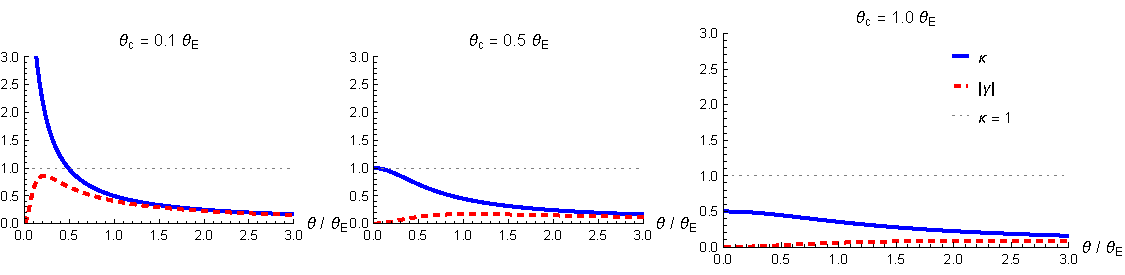
\includegraphics[width=0.85\textwidth]{../Figures/07_Axisymmetric_Models/nis_critical_curves.pdf}
    \caption{Effect of the core radius on the NIS convergence and
    shear, shown for three regimes that control the critical-curve
    topology.
    \textbf{Left:} for $\theta_c = 0.1\,\thetaE < \thetaE/2$, the
    central convergence $\kappab(0)>1$, so both tangential and radial
    critical curves exist and three images can form.
    \textbf{Center:} at the critical value $\theta_c = 0.5\,\thetaE =
    \thetaE/2$, $\kappab(0)=1$ exactly and the radial critical curve
    collapses to a point.
    \textbf{Right:} for $\theta_c = 1.0\,\thetaE > \thetaE/2$,
    $\kappab(0)<1$ everywhere; no critical curves exist and only one
    image forms.  Generated by
    \texttt{axisymmetric\_models.wl}.}
    \label{fig:nis_critical_curves}
\end{figure}


% =====================================================================
\section{NFW Profile}
\label{sec:nfw}

The \textbf{Navarro--Frenk--White} (NFW) profile is the ``universal''
dark matter halo density profile found in cosmological $N$-body
simulations (Navarro, Frenk \& White 1996, 1997).  It is the standard
model for the mass distribution of galaxy clusters and is essential
for cluster lensing (Module~10).

\subsection{Three-Dimensional Density Profile}

\begin{equation}
    \boxed{
    \rho(r) = \frac{\rho_s}{\left(\dfrac{r}{r_s}\right)
    \left(1 + \dfrac{r}{r_s}\right)^2}
    }
    \label{eq:nfw_rho}
\end{equation}
where $r_s$ is the \textbf{scale radius} and $\rho_s$ is a
characteristic density.  The profile has two regimes:
\begin{itemize}
    \item $r \ll r_s$: $\rho \propto r^{-1}$ (cusp, shallower than
          isothermal),
    \item $r \gg r_s$: $\rho \propto r^{-3}$ (steeper than
          isothermal, finite total mass within a virial radius).
\end{itemize}

\subsection{NFW Parameters: Concentration and Virial Mass}

The NFW profile is usually parametrized by two quantities:
\begin{itemize}
    \item The \textbf{virial mass} $M_{200}$: the mass enclosed
          within the virial radius $r_{200}$, defined as the radius
          within which the mean density is 200 times the critical
          density of the universe.
    \item The \textbf{concentration parameter}
          $c = r_{200}/r_s$: the ratio of virial to scale radius.
          Typical values are $c \sim 3$--$5$ for massive clusters
          ($M_{200} \sim 10^{15}\,\Msun$) and $c \sim 10$--$20$ for
          galaxy-mass haloes ($M_{200} \sim 10^{12}\,\Msun$).
\end{itemize}

The characteristic density is related to $c$ by:
\begin{equation}
    \rho_s = \frac{200}{3}\,\rho_{\mathrm{crit}}\,
    \frac{c^3}{\ln(1+c) - c/(1+c)} \,.
    \label{eq:nfw_rho_s}
\end{equation}

\subsection{Surface Mass Density of the NFW}
\label{sec:nfw_sigma}

The line-of-sight projection of the NFW density gives the surface mass
density
\begin{equation}
    \Sigma(\xi) \;=\; \int_{-\infty}^{\infty}
        \rho\!\left(\sqrt{\xi^2 + z^2}\right)\,dz \,,
    \label{eq:nfw_sigma_setup}
\end{equation}
where $\xi$ is the physical impact parameter in the lens plane and $z$
is the line-of-sight coordinate.  We now evaluate this integral
explicitly; the computation separates cleanly into three steps and is
the first place where the distinctive NFW branch structure
(arccosh vs.\ arctan) appears.  The full derivation is verified
symbolically in
\mathlink{07_Axisymmetric_Models/nfw\_projection.wl}{nfw\_projection.wl}.

\paragraph{Step 1: dimensionless variables.}
Let $x = \xi/r_s$ and $u = z/r_s$, so that $r/r_s = \sqrt{x^2+u^2}$ and
$dz = r_s\,du$.  The NFW density (eq.~\ref{eq:nfw_rho}) becomes
\begin{equation*}
    \rho = \frac{\rho_s}{\sqrt{x^2+u^2}\,\bigl(1 + \sqrt{x^2+u^2}\bigr)^2}\,.
\end{equation*}
Using the symmetry $z \leftrightarrow -z$,
\begin{equation}
    \Sigma(\xi) \;=\; 2\,\rho_s\,r_s\,I(x) \,,
    \qquad
    I(x) = \int_0^{\infty}\!
        \frac{du}{\sqrt{x^2+u^2}\,\bigl(1 + \sqrt{x^2+u^2}\bigr)^2}\,.
    \label{eq:nfw_I_definition}
\end{equation}

\paragraph{Step 2: change of variable $w = \sqrt{x^2+u^2}$.}
Then $u\,du = w\,dw$ and $du = w\,dw/\sqrt{w^2-x^2}$.  The limits
$u\!:\!0\to\infty$ map to $w\!:\!x\to\infty$, and
\begin{equation}
    I(x) \;=\; \int_{x}^{\infty}\!
        \frac{dw}{(1+w)^2\,\sqrt{w^2 - x^2}} \,.
    \label{eq:nfw_I_wform}
\end{equation}

\paragraph{Step 3: reduce to a simpler integral.}
A short calculation gives the identity
\begin{equation}
    \frac{d}{dw}\!\left[\frac{\sqrt{w^2-x^2}}{1+w}\right]
    \;=\;
    \frac{w + x^2}{(1+w)^2\sqrt{w^2-x^2}}\,.
    \label{eq:nfw_parts_identity}
\end{equation}
Writing $w + x^2 = (1+w) + (x^2 - 1)$ splits the right side into a
piece involving one power of $(1+w)$ in the denominator and the
target integrand $\bigl[(1+w)^2\sqrt{w^2-x^2}\bigr]^{-1}$ multiplied by
$(x^2-1)$.  Integrating eq.~\eqref{eq:nfw_parts_identity} from $w=x$ to
$w=\infty$ and using $\sqrt{w^2-x^2}/(1+w)\to 1$ at infinity and $0$ at
$w=x$:
\begin{equation}
    1 \;=\; K(x) \;+\; (x^2 - 1)\,I(x) \,,
    \qquad
    K(x) \equiv \int_x^{\infty}\!\frac{dw}{(1+w)\sqrt{w^2-x^2}}\,,
    \label{eq:nfw_IbK}
\end{equation}
so
\begin{equation}
    I(x) \;=\; \frac{1 - K(x)}{x^2 - 1}\,.
    \label{eq:nfw_I_as_K}
\end{equation}

\paragraph{Step 4: evaluate $K(x)$.}
The substitution $w = x\cosh\tau$ (with $\sqrt{w^2-x^2} = x\sinh\tau$,
$dw = x\sinh\tau\,d\tau$) turns $K$ into
\begin{equation}
    K(x) \;=\; \int_0^{\infty} \frac{d\tau}{1 + x\cosh\tau} \,,
    \label{eq:nfw_Ktau}
\end{equation}
which is elementary.  Using the Weierstrass half-angle substitution
$t = \tanh(\tau/2)$ and the standard result
$\int_0^1\! 2\,dt/(a-b\,t^2)
= (2/\sqrt{ab})\,\operatorname{arctanh}\!\sqrt{b/a}$
(and its arctan analog when the signs flip), one finds
\begin{equation}
    \boxed{
    K(x) = \begin{cases}
        \dfrac{\operatorname{arccosh}(1/x)}{\sqrt{1-x^2}},
            & 0 < x < 1, \\[8pt]
        1, & x = 1, \\[4pt]
        \dfrac{\arctan\!\sqrt{x^2-1}}{\sqrt{x^2-1}},
            & x > 1.
    \end{cases}}
    \label{eq:nfw_K_branches}
\end{equation}
The two branches are related by the identity
$\operatorname{arccosh}(1/x) \leftrightarrow \arccos(1/x)$ (analytic
continuation through $x=1$), and the $x=1$ value follows from a
Taylor expansion of either branch.

\paragraph{Collected result.}
Substituting eq.~\eqref{eq:nfw_K_branches} into
eq.~\eqref{eq:nfw_I_as_K}, and then eq.~\eqref{eq:nfw_I_definition},
\begin{equation}
    \boxed{
    \Sigma(x) = 2\,\rho_s\,r_s\, f(x)\,,
    \qquad
    f(x) = \frac{1 - K(x)}{x^2 - 1}\,,}
    \label{eq:nfw_sigma}
\end{equation}
where $x = \xi / r_s = \theta / \theta_s$ and $\theta_s = r_s / \Dd$.
Writing out the three branches explicitly,
\begin{equation}
    f(x) = \begin{cases}
    \dfrac{1}{x^2 - 1}\!\left(1 - \dfrac{\operatorname{arccosh}(1/x)}{\sqrt{1-x^2}}\right)
            & 0 < x < 1, \\[8pt]
    \dfrac{1}{3} & x = 1, \\[8pt]
    \dfrac{1}{x^2 - 1}\!\left(1 - \dfrac{\arctan\!\sqrt{x^2-1}}{\sqrt{x^2-1}}\right)
            & x > 1.
    \end{cases}
    \label{eq:nfw_f}
\end{equation}
This recovers the standard result of Bartelmann (1996) and
Wright \& Brainerd (2000).

\begin{remark}
The apparent singularity at $x = 1$ in eq.~\eqref{eq:nfw_f} cancels
between numerator and denominator.  A Taylor expansion of $1 - K(x)$
about $x = 1$ (for either branch) gives
$1 - K(x) = \tfrac{1}{3}(x^2 - 1) + \order{(x^2-1)^2}$, leaving
$f(1) = 1/3$ --- a smooth function of $x$.
\end{remark}

\subsection{Convergence of the NFW}

Dividing eq.~\eqref{eq:nfw_sigma} by the critical surface density,
\begin{equation}
    \boxed{
    \kappab(x) \;=\; \frac{\Sigma(x)}{\Sigmacr}
    \;=\; \frac{2\,\rho_s\,r_s}{\Sigmacr}\, f(x)
    \;\equiv\; \kappa_s\, f(x) \,,
    \qquad
    \kappa_s \equiv \frac{2\rho_s r_s}{\Sigmacr}.}
    \label{eq:nfw_kappa}
\end{equation}
The characteristic convergence $\kappa_s$ collects every
dimensionful quantity from the density profile and the distance
configuration, leaving $f(x)$ purely dimensionless.

\begin{remark}
Unlike the SIS (where $\kappab \propto \theta^{-1}$), the NFW
convergence has a \textit{logarithmic} divergence as $x \to 0$.  This
follows from the small-$x$ expansion of eq.~\eqref{eq:nfw_K_branches},
$\operatorname{arccosh}(1/x) = \ln(2/x) + \order{x^2}$, which gives
$K(x)\to \ln(2/x)$ and hence $f(x) \sim \ln(2/x)$ as $x\to 0$.  The
NFW cusp ($\rho \propto r^{-1}$) is shallower than the isothermal cusp
($\rho \propto r^{-2}$), which has important consequences for central
image formation.
\end{remark}

\subsection{Deflection Angle and Shear of the NFW}

For any axisymmetric profile, the reduced deflection angle satisfies
eqs.~\eqref{eq:mean_kappa} and~\eqref{eq:alpha_mean_kappa},
\begin{equation}
    \alpha(\theta) \;=\; \theta\,\bar\kappa(\theta) \,,
    \qquad
    \bar\kappa(\theta) = \frac{2}{\theta^2}\int_0^\theta
        \kappab(\theta')\,\theta'\,d\theta'.
    \label{eq:nfw_alpha_setup}
\end{equation}
Switching to $x = \theta/\theta_s$ and using
$\kappab = \kappa_s f(x)$ (eq.~\ref{eq:nfw_kappa}) turns the integral
into
\begin{equation}
    \bar\kappa(x) = \frac{2\kappa_s}{x^2}\,h(x) \,,
    \qquad
    h(x) \equiv \int_0^x f(x')\,x'\,dx'.
    \label{eq:nfw_hdef}
\end{equation}

\paragraph{Evaluation of $h(x)$.}
From eq.~\eqref{eq:nfw_I_as_K},
$f(x) = [1 - K(x)]/(x^2-1)$, where $K(x)$ is given by
eq.~\eqref{eq:nfw_K_branches}.  A direct calculation shows
\begin{equation}
    \frac{d}{dx}\!\left[\ln\!\tfrac{x}{2} + K(x)\right]
    \;=\; x\,f(x)
    \quad\text{for } 0 < x \neq 1,
    \label{eq:nfw_antiderivative}
\end{equation}
and, using
$\operatorname{arccosh}(1/x) = \ln(2/x) + \order{x^2}$ as $x \to 0$,
\begin{equation*}
    \lim_{x\to 0^+}\bigl[\ln(x/2) + K(x)\bigr] = 0 \,.
\end{equation*}
Hence
\begin{equation}
    h(x) \;=\; \ln\!\frac{x}{2} + g(x) \,,
    \qquad
    g(x) \equiv K(x),
    \label{eq:nfw_h_evaluated}
\end{equation}
with
\begin{equation}
    g(x) = \begin{cases}
        \dfrac{\operatorname{arccosh}(1/x)}{\sqrt{1-x^2}}, & 0 < x < 1, \\[6pt]
        1, & x = 1, \\[4pt]
        \dfrac{\arctan\!\sqrt{x^2-1}}{\sqrt{x^2-1}}, & x > 1.
    \end{cases}
    \label{eq:nfw_g}
\end{equation}

\paragraph{Deflection angle and shear.}
Substituting eq.~\eqref{eq:nfw_h_evaluated} into
eqs.~\eqref{eq:nfw_alpha_setup}--\eqref{eq:nfw_hdef} and using
$\theta = x\,\theta_s$:
\begin{equation}
    \boxed{
    \alpha(x) = \frac{2\kappa_s\,\theta_s}{x}\,
    \left[\ln\frac{x}{2} + g(x)\right],
    \qquad
    \bar\kappa(x) = \frac{2\kappa_s}{x^2}\,
    \left[\ln\frac{x}{2} + g(x)\right].}
    \label{eq:nfw_alpha}
\end{equation}
The tangential shear of any axisymmetric profile is
$|\gammaL(x)| = \bar\kappa(x) - \kappab(x)$
(cf.\ eq.~\ref{eq:gamma_circular}):
\begin{equation}
    |\gammaL(x)| \;=\; \frac{2\kappa_s}{x^2}
        \left[\ln\frac{x}{2} + g(x)\right]
        \;-\; \kappa_s\,f(x) \,.
    \label{eq:nfw_gamma}
\end{equation}
Every identity in this subsection --- the antiderivative
eq.~\eqref{eq:nfw_antiderivative}, the $x \to 0$ limit, and the
numerical consistency of eq.~\eqref{eq:nfw_alpha} with direct
integration of $\kappab$ --- is verified symbolically and numerically
in
\mathlink{07_Axisymmetric_Models/nfw\_projection.wl}{nfw\_projection.wl}.

\subsection{Role of Concentration in NFW Lensing}

The concentration parameter $c$ has a strong effect on the lensing
strength of an NFW halo:
\begin{itemize}
    \item Higher $c$ means more centrally concentrated mass, increasing
          the central convergence $\kappab(0)$ and making strong lensing
          more likely.
    \item For a fixed virial mass, increasing $c$ increases $\kappa_s$
          and decreases $\theta_s$, concentrating the lensing signal in
          a smaller angular region.
    \item Typical galaxy clusters ($c \sim 4$--$5$) are strong lenses
          for background sources at $z_s \gtrsim 1$, producing giant
          arcs with radii of $\sim 10''$--$30''$.
\end{itemize}

The NFW model will be applied extensively to cluster lensing in
Module~10.

\begin{figure}[ht]
    \centering
    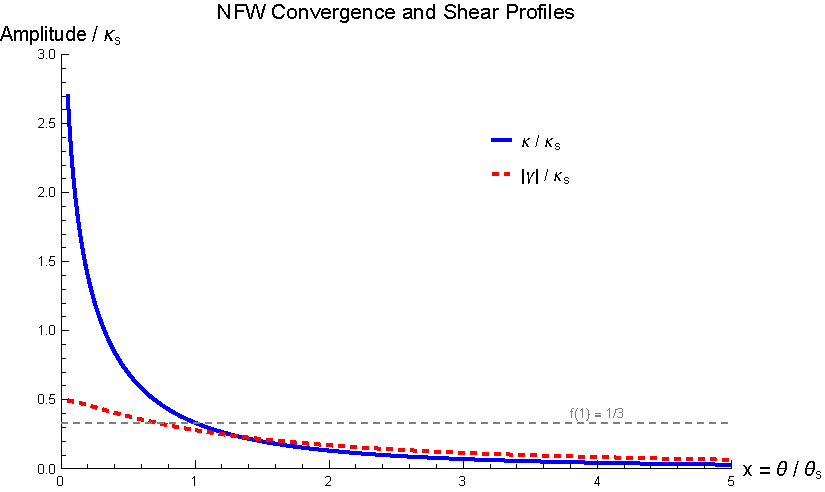
\includegraphics[width=0.75\textwidth]{../Figures/07_Axisymmetric_Models/nfw_profiles.pdf}
    \caption{NFW convergence $\kappab(x)/\kappa_s = f(x)$ (solid) and
    shear $|\gammaL(x)|/\kappa_s = \bar\kappa(x)/\kappa_s - f(x)$
    (dashed) as functions of the dimensionless radius $x = \theta/
    \theta_s$.  Both curves are normalized to $\kappa_s$ and are
    universal functions of $x$ (independent of concentration); the
    horizontal grey line marks $f(1) = 1/3$.  The concentration $c$
    enters only through the overall scale $\kappa_s$ and the angular
    scale $\theta_s$, both of which absorb the dependence on $c$ and
    on the cosmological distances.  Generated by
    \texttt{axisymmetric\_models.wl}.}
    \label{fig:nfw_profiles}
\end{figure}


% =====================================================================
\section{Comparison of Models}
\label{sec:model_comparison}

Table~\ref{tab:model_comparison} summarizes the key properties of the
four axisymmetric lens models covered in this module.

\begin{table}[ht]
\centering
\caption{Comparison of axisymmetric lens models.  Here
$\theta$ is the angular radius from the lens center in units of the
appropriate scale ($\thetaE$ for point mass and SIS, $\theta_s$ for
NFW).}
\label{tab:model_comparison}
\begin{tabular}{@{}lcccc@{}}
\toprule
Property & Point Mass & SIS & NIS & NFW \\
\midrule
$\rho(r)$ & $\delta^{(3)}$ & $\propto r^{-2}$ & $\propto (r^2+r_c^2)^{-1}$ & eq.~\eqref{eq:nfw_rho} \\[4pt]
$\kappab(\theta)$ & $0$ ($\theta \neq 0$) & $\thetaE / 2\theta$ & $\thetaE / 2\sqrt{\theta^2+\theta_c^2}$ & $\kappa_s\, f(x)$ \\[4pt]
$\alpha(\theta)$ & $\thetaE^2/\theta$ & $\thetaE$ & eq.~\eqref{eq:nis_alpha} & eq.~\eqref{eq:nfw_alpha} \\[4pt]
$\kappab = |\gammaL|$? & No ($\kappab=0$) & Yes & No & No \\[4pt]
Tangential CC & $\theta = \thetaE$ & $\theta = \thetaE$ & Yes & Yes \\[4pt]
Radial CC & No & No & Yes ($\theta_c < \thetaE/2$) & Yes \\[4pt]
Max images & 2 & 2 & 3 & 3 \\[4pt]
Caustic & Point & Point & Point $+$ circle & Point $+$ circle \\
\bottomrule
\end{tabular}
\end{table}

The key qualitative differences between the models are:

\begin{enumerate}
    \item \textbf{Central density:} The point mass and SIS have
          singular central densities; the NIS and NFW have finite (or
          logarithmically divergent) central densities.  The central
          density determines whether a radial critical curve can form.

    \item \textbf{Deflection angle behavior:} The point mass
          deflection $\alpha \propto 1/\theta$ diverges at the center
          and falls off with distance.  The SIS deflection is constant.
          The NIS and NFW deflections are intermediate.

    \item \textbf{Image multiplicity:} Models with a radial critical
          curve (NIS, NFW) can produce a third (central) image.  The
          SIS and point mass produce at most two images.

    \item \textbf{Asymptotic behavior:} The SIS has $\Sigma \propto
          \theta^{-1}$ and infinite total mass.  The NFW has
          $\Sigma \propto \theta^{-2}$ (for $\theta \gg \theta_s$) and
          a well-defined virial mass.
\end{enumerate}

\begin{figure}[ht]
    \centering
    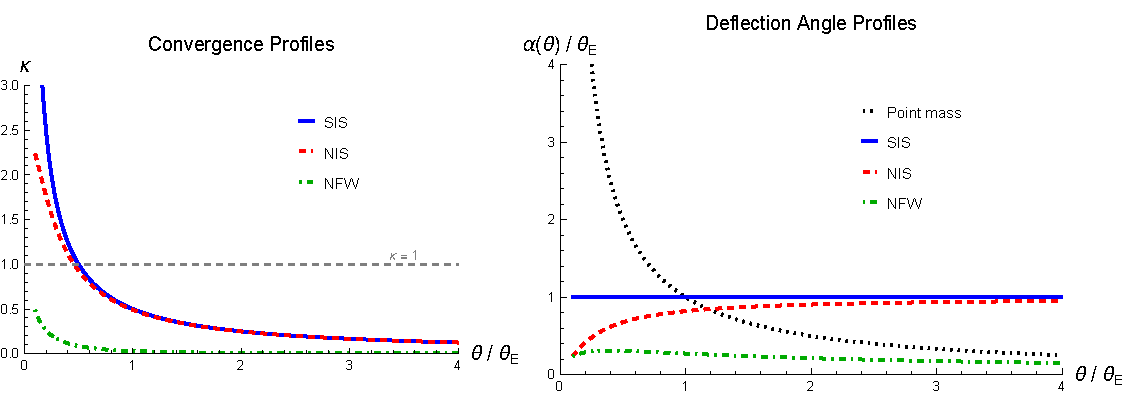
\includegraphics[width=0.85\textwidth]{../Figures/07_Axisymmetric_Models/model_comparison.pdf}
    \caption{Comparison of convergence profiles (left) and deflection
    angles (right) for the four axisymmetric models.  All curves use
    the SIS Einstein radius $\thetaE$ as the unit of length on the
    horizontal axis; the SIS, NIS and NFW amplitudes are set so that
    the profiles can be compared on the same panel
    (specifically NIS with $\theta_c = 0.2\,\thetaE$ and NFW with
    $\theta_s = 0.3\,\thetaE,\;\kappa_s = 0.5$).  Only the SIS and
    NIS are normalized to reproduce $\bar\kappa(\thetaE) = 1$; the
    NFW deflection therefore does not pass through $\alpha = \thetaE$
    at $\theta = \thetaE$ on this plot.  The point mass convergence
    is a delta function and is not shown.  Generated by
    \texttt{axisymmetric\_models.wl}.}
    \label{fig:model_comparison}
\end{figure}


% =====================================================================
\section{Summary}
\label{sec:axi_summary}

\begin{itemize}
    \item For a \textbf{circularly symmetric} lens, all quantities
          depend only on $\theta = |\vectheta|$.  The deflection angle
          is $\alpha(\theta) = \bar{\kappa}(\theta)\,\theta$, and the
          shear is $|\gammaL| = \bar{\kappa} - \kappab$.

    \item The \textbf{point mass} lens has $\alpha = \thetaE^2/\theta$,
          $\kappab = 0$ (away from origin), and always produces two
          images.

    \item The \textbf{SIS} has $\rho \propto r^{-2}$, a constant
          physical deflection angle
          $\alphahat = 4\pi\sigma_v^2/\speedoflight^2$, Einstein radius
          $\thetaE = 4\pi(\sigma_v/\speedoflight)^2\,\Dds/\Ds$, and
          $\kappab = |\gammaL| = \thetaE/(2\theta)$ everywhere.

    \item The SIS produces two images for $\beta < \thetaE$ and one
          image for $\beta > \thetaE$, with magnifications
          $\mu_\pm = 1 \pm \thetaE/\beta$.  It has a tangential
          critical curve (Einstein ring) but no radial critical curve.

    \item The \textbf{NIS} introduces a core radius $\theta_c$ that
          removes the central singularity.  For $\theta_c < \thetaE/2$,
          a radial critical curve appears, enabling a third (central)
          image.  The NIS reduces to the SIS for $\theta_c \to 0$.

    \item The \textbf{NFW} profile
          $\rho = \rho_s / [(r/r_s)(1+r/r_s)^2]$ is the universal dark
          matter halo profile.  It is parametrized by the virial mass
          $M_{200}$ and concentration $c$.  Higher concentration
          increases the lensing strength.

    \item Models with finite central density (NIS, NFW) possess a
          radial critical curve and can produce three images.  The
          SIS and point mass cannot.
\end{itemize}


% =====================================================================
\section{Problems}
\label{sec:axi_problems}

\begin{exercise}
\label{ex:sis_deflection_derivation}
\textbf{(Derivation of the SIS deflection angle.)}
Starting from the SIS density profile $\rho(r) = \sigma_v^2/(2\pi
\Gnewton r^2)$:
\begin{enumerate}[label=(\alph*)]
    \item Compute the surface mass density
          $\Sigma(\xi) = \int_{-\infty}^{+\infty}
          \rho(\sqrt{\xi^2 + z^2})\, dz$ and show that
          $\Sigma(\xi) = \sigma_v^2 / (2\Gnewton\,\xi)$.
          \textit{Hint:} Use the substitution $z = \xi\tan\phi$.
    \item Compute the projected enclosed mass
          $M(\xi) = 2\pi \int_0^\xi \Sigma(\xi')\,\xi'\,d\xi'$.
    \item Using $\alphahat(\xi) = 4\Gnewton M(\xi) /
          (\speedoflight^2\,\xi)$, show that
          $\alphahat = 4\pi\sigma_v^2/\speedoflight^2$, independent of
          $\xi$.
    \item Derive the SIS Einstein radius $\thetaE$.
\end{enumerate}
Verify with
\solnlink{07_Axisymmetric_Models/problems\_07.wl}{problems\_07.wl}.
\end{exercise}

\begin{exercise}
\label{ex:sis_kappa_equals_gamma}
\textbf{(SIS: $\kappab = |\gammaL|$ everywhere.)}
\begin{enumerate}[label=(\alph*)]
    \item For the SIS with $\kappab(\theta) = \thetaE/(2\theta)$,
          compute the mean convergence $\bar{\kappa}(\theta)$ using
          eq.~\eqref{eq:mean_kappa}.
    \item Show that $|\gammaL(\theta)| = \bar{\kappa}(\theta) -
          \kappab(\theta) = \thetaE/(2\theta) = \kappab(\theta)$.
    \item Explain physically why $\kappab = |\gammaL|$ for the SIS
          but $\kappab = 0 \neq |\gammaL|$ for the point mass.
          \textit{Hint:} Consider the mass distribution --- where is
          the mass located for each model?
    \item Show that for \textit{any} power-law profile
          $\kappab(\theta) \propto \theta^{-n}$ with $n > 0$, the
          ratio $|\gammaL|/\kappab$ is constant, and find the value of
          $n$ for which $|\gammaL| = \kappab$.
\end{enumerate}
Verify with
\solnlink{07_Axisymmetric_Models/problems\_07.wl}{problems\_07.wl}.
\end{exercise}

\begin{exercise}
\label{ex:sis_numerical}
\textbf{(SIS numerical example.)}
Consider an SIS lens with $\sigma_v = 250$~km\,s$^{-1}$ at
$z_d = 0.3$ lensing a source at $z_s = 1$.  Use
$\Dd \approx 920$~Mpc, $\Ds \approx 1650$~Mpc,
$\Dds \approx 1055$~Mpc.
\begin{enumerate}[label=(\alph*)]
    \item Compute the Einstein radius $\thetaE$ in arcseconds.
    \item For a source at $\beta = 0.5''$:
          \begin{enumerate}[label=(\roman*)]
              \item Is the source inside or outside the caustic?
              \item Find the image positions $\theta_+$ and $\theta_-$.
              \item Compute the magnifications $\mu_+$ and $\mu_-$.
              \item Compute the total magnification.
          \end{enumerate}
    \item For what source position $\beta$ does the SIS produce images
          with equal absolute magnification?  Is this physically
          realizable?
    \item Compare the SIS Einstein radius with the point mass Einstein
          radius for $M = 10^{12}\,\Msun$ at the same redshifts.
          Comment on the difference.
\end{enumerate}
Verify with
\solnlink{07_Axisymmetric_Models/problems\_07.wl}{problems\_07.wl}.
\end{exercise}

\begin{exercise}
\label{ex:nis_convergence}
\textbf{(NIS convergence and SIS limit.)}
\begin{enumerate}[label=(\alph*)]
    \item Starting from the NIS surface mass density
          $\Sigma(\theta) = \sigma_v^2 / [2\Gnewton\,\Dd\,
          \sqrt{\theta^2 + \theta_c^2}]$, derive the NIS convergence
          $\kappab(\theta) = \thetaE / [2\sqrt{\theta^2 + \theta_c^2}]$.
    \item Show that the NIS convergence reduces to the SIS convergence
          $\kappab = \thetaE/(2\theta)$ in the limit $\theta_c \to 0$.
    \item Find the critical value of $\theta_c$ (in terms of $\thetaE$)
          above which the NIS cannot produce multiple images.
          \textit{Hint:} multiple images require $\kappab(0) \geq 1$.
    \item For the NIS with $\theta_c = 0.1\,\thetaE$, compute
          $\kappab(0)$, $\kappab(\thetaE)$, and
          $\kappab(2\,\thetaE)$.
    \item Sketch (or plot) the NIS convergence profile for
          $\theta_c = 0$ (SIS), $\theta_c = 0.1\,\thetaE$,
          $\theta_c = 0.3\,\thetaE$, and $\theta_c = 0.5\,\thetaE$
          on the same axes.
\end{enumerate}
Verify with
\solnlink{07_Axisymmetric_Models/problems\_07.wl}{problems\_07.wl}.
\end{exercise}

\begin{exercise}
\label{ex:nfw_concentration}
\textbf{(NFW concentration and lensing strength.)}
\begin{enumerate}[label=(\alph*)]
    \item Using the NFW convergence formula
          $\kappab(x) = \kappa_s\,f(x)$ (eq.~\ref{eq:nfw_kappa}),
          plot $\kappab(x)/\kappa_s$ as a function of
          $x = \theta/\theta_s$ for $0.01 \leq x \leq 10$.
    \item For a cluster at $z_d = 0.3$ with $M_{200} = 10^{15}\,\Msun$
          and source at $z_s = 1$, compute $\kappa_s$ and $\theta_s$
          for $c = 5$, $c = 10$, and $c = 20$.
    \item Plot the convergence profiles $\kappab(\theta)$ (in arcsec)
          for the three concentrations on the same axes.  At what
          angular radius does $\kappab = 1$ for each case?
    \item Discuss how the concentration parameter affects:
          (i)~the Einstein radius, (ii)~the size of the region
          where $\kappab > 1$, and (iii)~the lensing cross-section
          for producing giant arcs.
\end{enumerate}
Use Mathematica to generate the plots.
See \mathlink{07_Axisymmetric_Models/axisymmetric_models.wl}{axisymmetric\_models.wl}
and \solnlink{07_Axisymmetric_Models/problems\_07.wl}{problems\_07.wl}.
\end{exercise}
